\documentclass{template/class}

\usepackage[T1]{fontenc}
\usepackage{parskip}

\usepackage{titlesec}
\titlespacing{\section}{0pt}{3.3ex}{2ex}
\titlespacing{\subsection}{0pt}{3.3ex}{1.65ex}
\titlespacing{\subsubsection}{0pt}{3.3ex}{1ex}
\usepackage{fancyhdr}
\fancyhf{}

\usepackage[
    colorlinks=true,
    linkcolor=black,
    anchorcolor=black,
    citecolor=black,
    filecolor=black,
    menucolor=black,
    runcolor=black,
    urlcolor=black
]{hyperref}

\usepackage{biblatex}
\bibliography{bibliography}

\usepackage{graphicx}
\graphicspath{{./images/}}
\usepackage{transparent}
\usepackage{eso-pic}

\usepackage{tabularx}
\usepackage{colortbl}
\usepackage{longtable}

\usepackage{amsthm}
\usepackage{fix-cm}
\usepackage{algorithm}

\newcommand\numfontsize{\@setfontsize\Huge{200}{60}}

\newcommand{\hsp}{\hspace{0pt}}

\makeatletter
\renewcommand*\cleardoublepage{
    \clearpage
    \if@twoside
        \ifodd\c@page\else\null
            \AddToShipoutPicture*\backgroundbl
            \thispagestyle{empty}\newpage
            \if@twocolumn
                \hbox{}
                \newpage
            \fi
        \fi
    \fi
}
\makeatother

\definecolor{polimiblue}{cmyk}{.4,.1,0,.4}

\titleformat{\chapter}[hang]{\fontsize{50}{20}\selectfont\bfseries\filright}{
    \textcolor{polimiblue}
    \thechapter\hsp\hspace{2mm}\textcolor{polimiblue}{|   }
    \hsp
}{0pt}{\huge\bfseries\textcolor{polimiblue}}

\titleformat{\section}
{\color{polimiblue}\normalfont\Large\bfseries}
{\color{polimiblue}\thesection.}{1em}{}

\titleformat{\subsection}
{\color{polimiblue}\normalfont\large\bfseries}
{\color{polimiblue}\thesubsection.}{1em}{}

\titleformat{\subsubsection}
{\color{polimiblue}\normalfont\large\bfseries}
{\color{polimiblue}\thesubsubsection.}{1em}{}

\captionsetup[table]{labelfont={color=polimiblue}}
\captionsetup[figure]{labelfont={color=polimiblue}}


\begin{document}

\frontmatter

\puttitle{
	title=Students\&Companies,
    subtitle=Requirements Analysis\\and Specification Document,
	authors=Andrea Carrara\\e Federica Currò Dossi,
	date=22nd of December 2024
}

\tableofcontents

\mainmatter
\setcounter{page}{1}

\chapter{Introduction}
This chapter provides essential background information about the design document, including its purpose, scope and structure.
It also introduces key terminology and references needed for understanding the technical content that follows.

\section{Purpose}
The purpose of the following document is to present a detailed design description of Students\&Companies.
It provides developers with implementation guidelines while serving as a technical agreement between customers and contractors.
The document transforms the requirements and specifications from the requirements analysis and specification document \cite{carraracurrodossi2024} into concrete architectural decisions, describing the system's components and their interactions.
It outlines the design patterns, technical interfaces and deployment strategies that will guide the development team in building a robust platform that fulfills stakeholder needs.
Additionally, it establishes a clear roadmap for implementation and testing phases, ensuring that the final system aligns with both technical requirements and business objectives.

\section{Scope}
Students\&Companies is designed to bridge the gap between academic education and practical workplace experience.
The platform facilitates the internship matching process by enabling students to create detailed profiles with CVs and preferences, while companies can post comprehensive internship opportunities including project details, required skills and terms.
S\&C features personalized recommendations through statistical analysis, manages the entire selection process from interviews to final outcome and provides tools for monitoring ongoing internships.
Additionally, universities can oversee the progress of their students, ensuring quality and addressing concerns that arise during the internships.
For a comprehensive overview of the platform's functionalities and requirements, please refer to the requirements analysis and specification document \cite{carraracurrodossi2024}.

\section{Glossary}
This table contains the key definitions, acronyms and abbreviations used in the document.

\renewcommand{\arraystretch}{1.5}
\begin{longtable}{|c|p{8.5cm}|}
    \hline \rowcolor{polimiblue!40}
    \textbf{ID} & \textbf{Description} \\ \hline
    S\&C & Students\&Companies \\ \hline
    US & University student \\ \hline
    IN & Internship job \\ \hline
    PO & Internship position \\ \hline
    CO & Company \\ \hline
    UN & University \\ \hline
    CV & Curriculum vitae \\ \hline
    Match & A US and a CO declare interest in each other \\ \hline
    Contact & Selection process and internship progress \\ \hline
\caption{Glossary}
\end{longtable}

\section{Reference Documents}
The document follows Professor Di Nitto's project assignment structure \cite{dinitto2024}.

\section{Document Structure}
This document describes the design specification for Students\&Companies, following an architecture-centric approach that progresses from system-wide design decisions to specific implementation details.
It is organized into seven chapters, each providing increasingly detailed technical information needed for implementation.

\subsubsection{Introduction}
The first chapter establishes the foundation of the design document through purpose and scope definitions, provides a comprehensive glossary, lists reference documents and explains the document's organization.

\subsubsection{Architectural Design}
The second chapter presents the system's architecture through multiple views: an overview of components and their interactions, detailed component descriptions, deployment specifications, runtime behavior illustrations, component interfaces and the rationale behind architectural styles and patterns.

\subsubsection{User Interface Design}
The third chapter details the user interface through mockups and interaction flows, covering each user category's specific interface requirements and presenting key screens and navigation patterns.

\subsubsection{Requirements Traceability}
The fourth chapter establishes clear links between the requirements from the requirements analysis and specification document \cite{carraracurrodossi2024} and their corresponding design elements, demonstrating how architectural decisions satisfy functional and non-functional requirements.

\subsubsection{Implementation, Integration and Test Plan}
The fifth chapter provides a comprehensive roadmap for system realization, detailing the implementation order of components, their integration strategy and the testing methodology to ensure system quality.

\subsubsection{Workload}
The sixth chapter quantifies each writer's time investment in the design document.


\chapter{Overall Description}
This chapter provides a detailed description of the whole problem, offering a deeper exploration of the domain through various scenarios and the application of class and state diagrams.
It also covers key aspects such as product and user characteristics, as well as the underlying assumptions and constraints shaping the context.

\section{Product Perspective}
This section employs scenarios to illustrate the platform's role, supported by class and state diagrams that define its structure and dynamic behavior.
These tools collectively establish a clear understanding of how the product integrates into its environment and addresses the identified problem.

\subsection{Scenarios}
\newcounter{s}
\setcounter{s}{1}
\newcommand{\sco}{\thes\stepcounter{s}}

\subsubsection*{S\sco. Signup and Profile Setup}
AlgoSphere is a company specializing in algorithm development and artificial intelligence solutions for businesses across industries.
To cultivate fresh talent and build a pipeline of future employees, the company is considering offering several internship positions.
To save valuable time and resources, AlgoSphere opts to use Students\&Companies.
It navigates to the S\&C platform via a browser, selects the option "Sign Up as a Company"
and provides its name, email and field of operation.

Ben Pinter, a first-year Master's student in computer science, is eager to gain real-world experience in AI through an internship.
To streamline his search and avoid the inefficiency of navigating multiple websites and job boards, Ben signs up on S\&C, hoping to find opportunities aligned with his academic background and career goals.
Accessing the platform via a browser, he selects the "Sign Up as a Student" option and completes his profile by providing essential details, including his name, surname and email.
He also has the option to add information such as his CV and personal preferences.
These preferences may include availability, expected salary and benefits.

TechVille University, where Ben is currently enrolled, recognizes the importance of staying involved in students’ professional development to ensure they gain valuable experience and meet academic standards.
To facilitate this, TechVille University signs up on S\&C by selecting "Sign Up as a University" and providing its name and email.
By linking Ben’s profile to the university through his institutional email, the platform allows TechVille University to automatically monitor Ben’s internships, ensuring alignment with educational goals and providing support throughout his professional journey.

\subsubsection*{S\sco. Internship Posting and Candidate Matching}
AlgoSphere wants to post an internship position in AI. It clicks the corresponding button and describes the opportunity by outlining its tasks, application domain, project scope and offered terms such as salary and benefits.
After publishing, S\&C recommends Ben’s profile on AlgoSphere’s homepage, as his skills and experience closely match the internship requirements.
In turn, the platform notifies Ben about the opportunity.

Meanwhile, John Kent, another student in computer science, is registered on the platform but has not uploaded his CV or specified preferences.
Interested in artificial intelligence systems for cybersecurity, John uses the search bar to look for relevant opportunities by entering "AI."
Among the results, he finds AlgoSphere’s internship and applies, which prompts a notification to AlgoSphere.
To strengthen his application and improve his chances of being selected, John uploads his CV and specifies preferences.

\subsubsection*{S\sco. Selection Process}
After being notified, both Ben and AlgoSphere accept S\&C's recommendation, formally initiating contact and starting the selection process.
Similarly, upon reviewing John’s application, the company determines that his profile merits consideration.
The platform thus notifies John of the start of the selection process.

AlgoSphere uploads questionnaires tailored to the internship position, prompting notifications to both Ben and John to complete them.
When one submits them, the platform notifies AlgoSphere of the update and allows the company to view the answers.

After evaluating the questionnaires, AlgoSphere selects Ben as the stronger candidate due to his more aligned skills.
John is notified of his rejection, while Ben receives a notification detailing the next steps.
AlgoSphere then schedules a remote interview over an in-person one for better flexibility, which Ben accepts.
After a successful interview, the company finalizes the outcome of the selection process and notifies Ben, all through S\&C.

\subsubsection*{S\sco. Internship Monitoring}
Throughout Ben's internship, AlgoSphere will use S\&C to provide detailed progress reports or other comments, with notifications keeping Ben and his university informed of these updates in real time.
In turn, if Ben will encounter an issue during his time at AlgoSphere, such as unclear expectations from the company, he will comment a complaint visible to both AlgoSphere and TechVille University.

\subsubsection*{S\sco. Feedback Forms}
At key stages of the matchmaking, selection and internship processes, Ben and AlgoSphere will be asked to provide feedback on the quality of the service offered by S\&C.
Ben will share comments with respect to the quality of the recommendations he received and the efficiency of the selection process he completed.
In the same way, AlgoSphere will evaluate the platform's ability to provide suitable candidate matches, the usability of the system during selection and the effectiveness of its communication tools.

\subsection{Class Diagram}
The high-level class diagram below represents the entire system, modeling the elements from the previous scenarios along with their interactions and cardinalities.

\begin{figure}
    \centering
    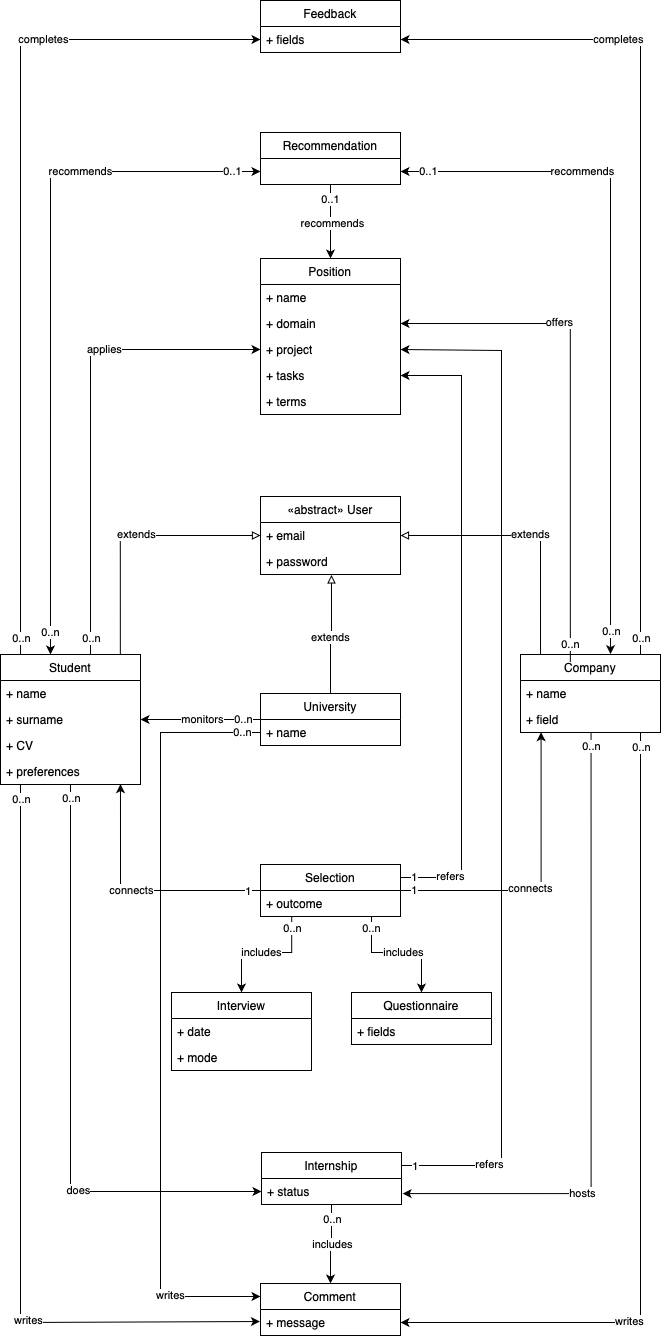
\includegraphics[width=10cm]{images/class-diagram.png}
    \caption{Class diagram}
\end{figure}

\subsection{State Diagrams}
The two state diagrams below aim to clarify potential misunderstandings about the recommendations and selection process by illustrating their dynamic behavior.

\subsubsection{Recommendations}
Recommendations are initiated when a company posts an internship position or a university student uploads their CV or personal preferences.
S\&C then checks for potential matches between available internship positions and student profiles.
Upon finding a match, the platform notifies the student about the position and the company about the student.
Each party can choose to accept or reject the recommendation.
If either party rejects it, the system resumes the search for another match.
However, if both accept, the system finalizes the match and notifies both the student and the company accordingly.

\begin{figure}
    \centering
    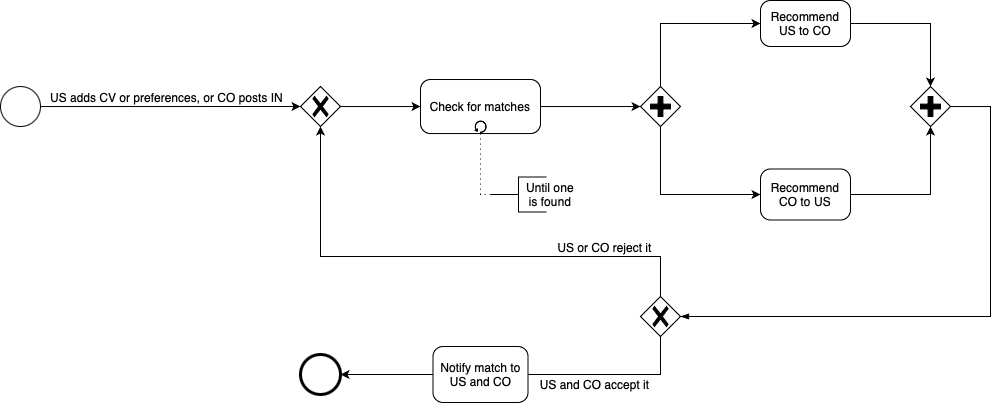
\includegraphics[width=14cm]{images/state-diagrams/recommendations.png}
    \caption{Recommendations state diagram}
\end{figure}

\subsubsection{Selection Process}
The selection process begins when a match is made between a university student and a company.
This happens either through mutual acceptance of a recommendation or when a student applies for an internship and the company accepts his application.
Once this connection is made, the system notifies both parties about the match.

From there, the company can choose to either add a questionnaire for the student or schedule an interview.
If an interview is scheduled, the student can accept or decline it.
After reviewing the questionnaire or evaluating the interview, the company decides whether to continue by sending another questionnaire or scheduling further interviews, or to conclude the process, notifying the student of the final outcome.

\begin{figure}
    \centering
    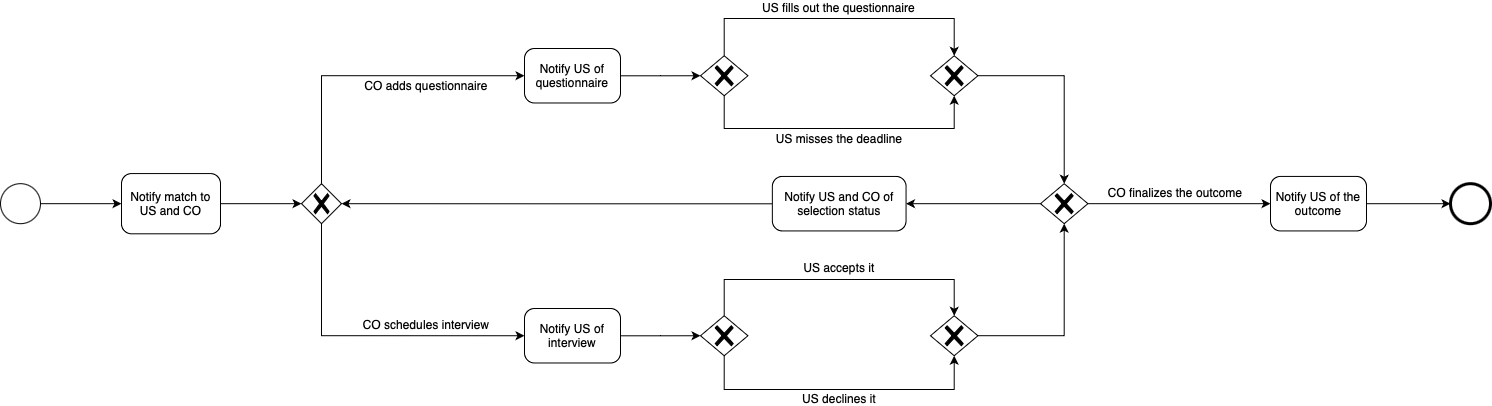
\includegraphics[width=16cm]{images/state-diagrams/selection-process.png}
    \caption{Selection process state diagram}
\end{figure}

\section{Product Functions}
The following is a summary of the main functions of Students\&Companies, providing a concise abstraction and generalization of its goals and scenarios.
This serves as an intermediate step bridging goals and scenarios with requirements and use cases.

\newcounter{f}
\setcounter{f}{1}
\newcommand{\fc}{\thef\stepcounter{f}}

\subsubsection*{F\fc. Signup and Profile Setup}
Students sign up with their name, surname and institutional email.
Additionally, they can upload a CV and set preferences.
Similarly, a company signs up by providing its name, email and field of operation, while universities do so by submitting their name and institutional email.
Students with the same institutional email domain are automatically linked to the university, allowing seamless monitoring.
After logging in, users can log out from their session and must log in again to reaccess the platform.

\subsubsection*{F\fc. Internship Posting and Searching}
Companies post internships by specifying their tasks, application domain, project scope and terms.
In turn, students write keywords in the search bar to find positions.

\subsubsection*{F\fc. Internship Application}
Students apply for internships and notifications are sent to companies, which can in turn review candidates’ profiles and start the selection process.

\subsubsection*{F\fc. Recommendations}
Students are recommended internship positions from suitable companies, while companies are recommended students based on skills and preferences.
Both students and companies must accept a recommendation to start the selection process.

\subsubsection*{F\fc. Selection Process}
Companies assess students through questionnaires and scheduled interviews, either virtual or in-person.
They then finalize the outcome, with notifications keeping both parties informed at every stage.

\subsubsection*{F\fc. Internship Monitoring}
Students, companies and universities are notified of the status of the ongoing internship and can write comments to share progress or raise concerns.

\subsubsection*{F\fc. Feedback Forms}
Students and companies provide feedback on matchmaking to refine the statistical analysis on which recommendations are based.

\section{User Characteristics}
Students\&Companies has three types of users: university students, companies and universities.
Below is a brief explanation of their identities and main characteristics.

\subsubsection{University Students}
University students are the users seeking internships.
A student can sign up by providing his name, surname and valid institutional email address in his personal data.
They can also upload a CV and specify personal preferences, such as availability and desired benefits.

\subsubsection{Companies}
Companies are the users hosting internships and they are typically represented by the human resources department acting on behalf of the organization.
Signing up requires the company's name, a valid email address and its field of expertise.

\subsubsection{Universities}
Universities are the users monitoring their students and they are typically represented by the career services department acting on behalf of the institution.
Signing up requires the university's name and a valid institutional email address.

\section{Assumptions and Constraints}
The table below outlines the domain assumptions of Students\&Companies:

\newcounter{da}
\setcounter{da}{1}
\newcommand{\dac}{\theda\stepcounter{da}}
\renewcommand{\arraystretch}{1.5}
\begin{longtable}{|c|p{12.5cm}|}
    \hline \rowcolor{polimiblue!40}
    \textbf{ID} & \textbf{Description} \\ \hline \hline
    DA\dac & USs have a valid institutional email. \\ \hline
    DA\dac & COs have a valid email. \\ \hline
    DA\dac & UNs have a valid institutional email. \\ \hline
    DA\dac & USs have a working device with a reliable internet connection. \\ \hline
    DA\dac & COs have a working device with a reliable internet connection. \\ \hline
    DA\dac & UNs have a working device with a reliable internet connection. \\ \hline
\caption{Domain assumptions}
\end{longtable}

The following table lists the constraints of S\&C: 

\newcounter{c}
\setcounter{c}{1}
\newcommand{\cc}{\thec\stepcounter{c}}
\renewcommand{\arraystretch}{1.5}
\begin{longtable}{|c|p{12.5cm}|}
    \hline \rowcolor{polimiblue!40}
    \textbf{ID} & \textbf{Description} \\ \hline \hline
    C\cc & S\&C cannot prevent a CO from posting a PO. \\ \hline
    C\cc & S\&C cannot prevent a US from applying for a PO. \\ \hline
    C\cc & S\&C cannot prevent a UN from monitoring its US. \\ \hline
    C\cc & S\&C cannot declare a match if neither the CO evaluated positively the application of a US nor a recommendation was accepted by both. \\ \hline
    C\cc & S\&C cannot start a selection process before a match. \\ \hline
    C\cc & S\&C cannot end a selection process before an outcome. \\ \hline
    C\cc & S\&C cannot start an IN before the end of a selection process. \\ \hline
\caption{Constraints}
\end{longtable}


\chapter{Specific Requirements}
\chapter{Formal Analysis}
\chapter{Effort Spent}

\printbibliography

\listoffigures

\listoftables

\cleardoublepage

\end{document}
